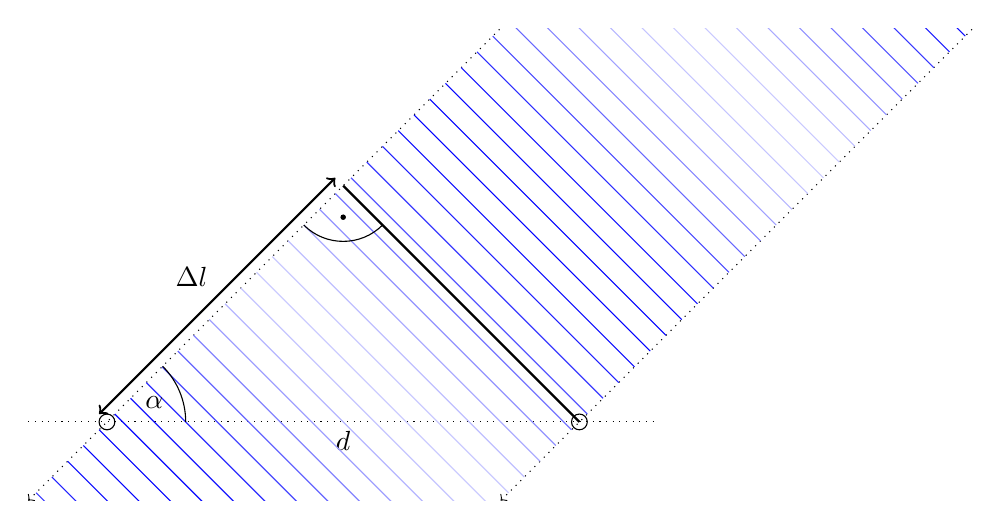
\begin{tikzpicture}
  % antennas
  \draw
  (-3, 0) circle(0.1)
  ( 3, 0) circle(0.1);

  % antenna normal
  \draw[dotted] (-4, 0) -- (4, 0);
  \draw (0, 0) node[below]{$d$};

  % signal rays
  \draw[dotted, <-] (-4, -1) -- +(6, 6);
  \draw[dotted, <-] ( 2, -1) -- +(6, 6);

  % train tracks
  \begin{scope}
    \clip
    (-4, -1) rectangle (8, 5);

    \foreach \x in{-4.5, -4.3, ..., 6}
      \pgfmathsetmacro\k{40*sin(1.5*\x r) + 60}
      \draw[color=blue!\k!white]
      ({3 + \x}, {\x}) -- +(-3, 3);
  \end{scope}

  % phase normal
  \draw[thick] (3, 0) -- +(-3, 3);
  \draw[thick, <->] (-3.1, 0.1) -- +(3, 3);
  \draw (-1.6, 1.6) node[above left]{$\Delta l$};

  % 90° mark
  \draw (-0.5, 2.5) arc (225:315:0.707);
  \fill (0, 2.6) circle(0.035);

  % unkown angle mark
  \draw
  (-2, 0) arc (0:45:1)
  (-2.4, 0.25) node[anchor=center]{$\alpha$};
\end{tikzpicture}
